\documentclass[conference]{IEEEtran}

% Text extraction (arXiv, indexers, screen readers): map ligatures to their letters
% and use T1 encoding under pdfLaTeX; XeTeX and LuaTeX handle this natively.
\usepackage{iftex}
\ifPDFTeX
  \input{glyphtounicode}
  \pdfgentounicode=1
  \usepackage[T1]{fontenc}
\fi

\usepackage{amsmath,amssymb}
\usepackage{graphicx}
\usepackage{booktabs}
\usepackage{multirow}
\usepackage{array}
\usepackage{cite}
\usepackage{xcolor}
\usepackage{url}
\usepackage{algorithm}
\usepackage[noend]{algpseudocode}
\usepackage{tikz}
\usetikzlibrary{arrows.meta,positioning,fit}
\usepackage[hidelinks]{hyperref}

\definecolor{auditblue}{HTML}{2A6F97}
\definecolor{auditred}{HTML}{C43C4E}
\definecolor{auditgreen}{HTML}{315B55}
\newcommand{\meanpm}[2]{#1\,$\pm$\,#2}
\newcommand{\protocol}[1]{\textsf{#1}}
% Plain text: synthesized small caps extract as "CytoF air".
\newcommand{\cytofair}{CytoFair}
\newcommand{\placeholder}[1]{\texttt{[#1]}}
\setlength{\textfloatsep}{7pt plus 1pt minus 2pt}
\setlength{\dbltextfloatsep}{7pt plus 1pt minus 2pt}
\setlength{\floatsep}{6pt plus 1pt minus 2pt}
\setlength{\dblfloatsep}{6pt plus 1pt minus 2pt}
\setlength{\abovecaptionskip}{3pt}
\setlength{\belowcaptionskip}{0pt}
\renewcommand{\arraystretch}{0.95}

\title{Do We Train on Test Cells? Provenance Leakage in Public Cervical Cytology Benchmarks}

\author{
\IEEEauthorblockN{Snehasish Ghosh\IEEEauthorrefmark{1},
Soham Mitra\IEEEauthorrefmark{2}, and
Nibaran Das\IEEEauthorrefmark{2}}
\IEEEauthorblockA{\IEEEauthorrefmark{1}Indian Institute of Science, Bengaluru, India\\
Email: snehasishg@iisc.ac.in}
\IEEEauthorblockA{\IEEEauthorrefmark{2}Department of Computer Science and Engineering,
Jadavpur University, Kolkata, India\\
Emails: \placeholder{SOHAM EMAIL}, \placeholder{NIBARAN EMAIL}}
}

\begin{document}
\maketitle

\begin{abstract}
Public cervical cytology benchmarks are built by cropping many cells from far fewer microscopic fields, and the literature splits them at the crop level.
We recover the concealed hierarchy and measure what that costs.
Under the standard stratified 80:20 crop split of SIPaKMeD, \meanpm{92.62}{0.40}\% of test crops have a training parent and \meanpm{52.62}{1.97}\% share literal source pixels with a training crop; CRIC reaches \meanpm{99.97}{0.08}\%, while single-cell Herlev returns exactly \meanpm{0.00}{0.00}\% and so serves as a negative control on the measurement itself.
The shortcut is learnable: a parent-identity probe reaches \meanpm{25.73}{0.66}\% on a 424-way task against a 0.2358\% chance baseline and a \meanpm{0.17}{0.24}\% label-shuffled comparator, and still reaches \meanpm{18.68}{1.25}\% from inpainted background alone---so the fingerprint is acquisition context, not cell morphology.
Correcting the evaluation unit lowers accuracy for all six architectures tested (\meanpm{0.72}{0.83} to \meanpm{2.25}{1.63} points, mean 1.37), an effect exceeding the 0.62-point spread between the two strongest published five-class results, though our five-seed per-architecture design is underpowered to certify individual contrasts after correction.
Adding near-duplicate purging on top of parent grouping produces no detectable further change, indicating that parent grouping alone is sufficient.
We release \cytofair: exact provenance maps, fixed parent-disjoint splits, and the audit toolkit, at \placeholder{REPOSITORY URL}.
\end{abstract}

\begin{IEEEkeywords}
cervical cytology, data leakage, provenance, grouped splitting, benchmark audit, reproducibility
\end{IEEEkeywords}

\section{Introduction}
Cervical cytology is a high-volume screening task in which a small number of abnormal cells must be recognized among many visually plausible normal cells.
The public-health burden is substantial: cervical cancer caused an estimated 660,000 new cases and 350,000 deaths worldwide in 2022, ranking fourth in both incidence and mortality among women~\cite{who2025hpv}.
Computer-assisted screening is therefore attractive not merely as a leaderboard problem, but as a way to support scarce expert attention.

That promise rests on an elementary validity condition: the held-out sample should represent genuinely unseen biological or acquisition units.
The image presented to a network is not always that unit.
Public cervical benchmarks are overwhelmingly \emph{cropped-from-parent} constructions---many cell images derived from far fewer microscopic fields.
Sibling crops from one field inherit stain batch, illumination, focus, background texture, preparation artifacts, and sometimes overlapping pixels.
A crop-level split then places siblings on both sides of evaluation while appearing formally disjoint at the filename level, because parent identifiers are not always carried into the released crop folders.

Whether this matters quantitatively depends on the scale of the effect relative to the differences the field publishes about.
That comparison is unusually stark here.
Deep learning has substantially advanced cervical-cell analysis: DeepPap classified cells directly and reported 98.3\% accuracy on Herlev~\cite{zhang2017deeppap}; DeepCervix fused multi-network features and reported 99.14\% five-class accuracy on SIPaKMeD~\cite{rahaman2021deepcervix}; a knowledge-distillation framework reported 98.52\% on the same task~\cite{gao2022knowledge}.
The two strongest five-class SIPaKMeD results we cite therefore differ by \textbf{0.62 percentage points}.
Any protocol artifact of comparable magnitude is not a footnote; it is larger than the quantity the literature is competing over.

These methods draw on residual, dense, efficient, mobile, and transformer backbones whose general image-recognition capabilities are well established~\cite{he2016resnet,huang2017densenet,sandler2018mobilenetv2,tan2019efficientnet,dosovitskiy2021vit}, and public resources made the comparisons possible: SIPaKMeD provides 4,049 cell crops derived from 966 cluster fields~\cite{plissiti2018sipakmed}, Cx22 provides 1,320 generated regions with instance labels~\cite{liu2022cx22}, CRIC provides 11,534 classified cells in 400 source images~\cite{rezende2021cric}, and Herlev provides 917 single-cell images~\cite{jantzen2005pap}.
Performance engineering has advanced faster than auditing of the sampling hierarchy beneath these released observations.

This work recovers that hierarchy exactly where the release permits it, measures what crop splitting shares, tests whether the shared signal is learnable, and constructs partitions that keep a parent---and, in a conservative sensitivity analysis, a near-duplicate component---wholly in one arm.
We separate two claims throughout, because only one of them is established here: recoverable parent information shows a shortcut is \emph{available}, not that every class model exploits it.

Our contributions are fivefold:
\begin{itemize}
    \item \cytofair, an auditable framework for exact crop-to-parent recovery, deterministic fail-closed validation, and provenance-aware split generation;
    \item the first complete dual-branch provenance map for all 4,049 SIPaKMeD crops---two independent recoveries agreeing on 4,049/4,049---together with subset-level source recovery for Cx22 and structural audits of CRIC and Herlev;
    \item a structural negative control: single-cell Herlev returns exactly zero on every leakage endpoint, validating the measurement instrument rather than only the datasets under test;
    \item direct measurement of parent straddling, literal cross-split pixel sharing, and a five-seed parent-identity probe with four transformation controls and a shuffled-label comparator, localizing the fingerprint to acquisition context;
    \item fixed parent-disjoint splits, released, with a deliberately bounded report of downstream accuracy sensitivity on SIPaKMeD---the one dataset given the full six-architecture rescore---and evidence that the cheaper grouping criterion suffices.
\end{itemize}

\section{Related Work}
\subsection{Cervical Cell Classification}
Crop-level cervical classification is mature.
Zhang \emph{et al.} established that direct CNN classification of cell images was viable, reporting 98.3\% on Herlev~\cite{zhang2017deeppap}.
Rahaman \emph{et al.} pushed five-class SIPaKMeD accuracy to 99.14\% through hybrid feature fusion~\cite{rahaman2021deepcervix}, and Gao \emph{et al.} reached 98.52\% on the same task via transfer learning and knowledge distillation~\cite{gao2022knowledge}.
We do not import these accuracies into our own comparison, because nominally identical datasets under different splits do not define comparable tests.
We do use their \emph{spread}: the 0.62-point interval separating the two strongest results calibrates how large a protocol effect has to be before it matters.

\subsection{What This Study Inherits}
Our design is assembled from four established lines of work rather than proposed from scratch.

Barz and Denzler supply the template: audit a benchmark for train--test near-duplicates, quantify the exposure, and release a corrected evaluation set rather than only a complaint.
They identified training counterparts for 3.3\% and 10\% of CIFAR-10 and CIFAR-100 test images and published ciFAIR~\cite{barz2020cifair}.
We follow that pattern, substituting exactly recovered provenance for image similarity as the grouping criterion, and reserving similarity for a labeled sensitivity analysis.

Laroca \emph{et al.} supply the re-evaluation protocol: after constructing duplicate-free splits for license-plate recognition, they re-ran six recognition models to characterize how conclusions move~\cite{laroca2023lpr}.
Our \protocol{P1}/\protocol{P2}/\protocol{P3} comparison across six backbones is the same manoeuvre in a medical-imaging setting.

Packh\"auser \emph{et al.} supply the mechanism instrument.
Their demonstration that chest radiographs support patient re-identification at 95.55\% accuracy on ChestX-ray14~\cite{packhauser2022reidentification} establishes identity probing as a way to show that a nuisance signal is \emph{present and learnable}, independent of any downstream task.
Section~\ref{sec:probe} adapts it from patient identity to source-field identity, and adds the transformation ablation needed to localize the substrate.

Kapoor and Narayanan supply the taxonomy, situating train--test non-independence within a broader account of leakage and reproducibility failure across ML-based science~\cite{kapoor2023leakage}.
Their vocabulary lets us name the specific failure precisely rather than describe it.

Table~\ref{tab:prior} records what each line contributes here.
The remaining gap is an exact, validated provenance audit and a corrected public evaluation resource for cervical-cytology crop benchmarks; this paper supplies it.

\begin{table*}[t]
\caption{Lineage of the present design. Each row records what this study takes from prior work, not a deficiency in it.}
\label{tab:prior}
\centering
\scriptsize
\setlength{\tabcolsep}{8pt}
\begin{tabular}{p{0.17\textwidth}p{0.15\textwidth}p{0.19\textwidth}p{0.36\textwidth}}
\toprule
Work & Method / audit & Reported result & What this study inherits \\
\midrule
DeepPap~\cite{zhang2017deeppap} & Direct CNN & 98.3\% Herlev & Establishes crop-level classification as the standard task formulation \\
DeepCervix~\cite{rahaman2021deepcervix} & Feature fusion & 99.14\% SIPaKMeD & Upper end of the published five-class range \\
Gao \emph{et al.}~\cite{gao2022knowledge} & Distillation & 98.52\% SIPaKMeD & Second reference point; with the row above, fixes the 0.62-point competitive spread \\
ciFAIR~\cite{barz2020cifair} & Duplicate audit & 3.3/10\% test duplicates & Audit-quantify-release template; corrected-benchmark publication model \\
Laroca \emph{et al.}~\cite{laroca2023lpr} & Fair LPR splits & Six models re-evaluated & Multi-architecture re-evaluation protocol under corrected splits \\
Packh\"auser \emph{et al.}~\cite{packhauser2022reidentification} & Identity probe & 95.55\% ChestX-ray14 & Identity probing as evidence that a nuisance signal is learnable \\
Kapoor \& Narayanan~\cite{kapoor2023leakage} & Leakage taxonomy & --- & Formal vocabulary for train--test non-independence \\
\bottomrule
\end{tabular}
\end{table*}

\section{Method}
Figure~\ref{fig:pipeline} summarizes the pipeline.
\cytofair{} treats provenance recovery as a prerequisite, not a post-hoc clustering step: released or exactly reconstructed parent identity defines the independent grouping unit, while image-derived similarity is reserved for a separately labeled sensitivity protocol.

\begin{figure*}[t]
\centering
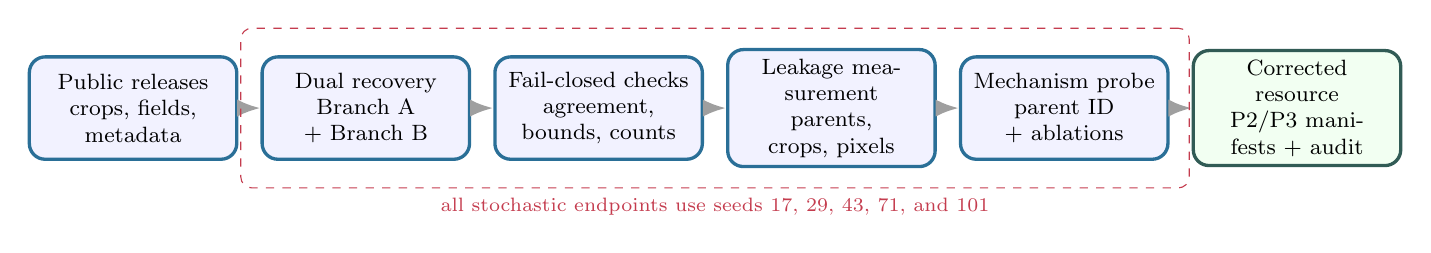
\begin{tikzpicture}[
    node distance=2.8mm,
    >=Latex,
    stage/.style={draw=auditblue, very thick, rounded corners=2mm, fill=blue!5,
                  minimum height=13mm, text width=24mm, align=center, font=\footnotesize},
    result/.style={draw=auditgreen, very thick, rounded corners=2mm, fill=green!5,
                  minimum height=13mm, text width=24mm, align=center, font=\footnotesize},
    arrow/.style={->, very thick, draw=gray!75}
]
\node[stage] (release) {Public releases\\crops, fields, metadata};
\node[stage, right=of release] (recover) {Dual recovery\\Branch A + Branch B};
\node[stage, right=of recover] (validate) {Fail-closed checks\\agreement, bounds, counts};
\node[stage, right=of validate] (measure) {Leakage measurement\\parents, crops, pixels};
\node[stage, right=of measure] (probe) {Mechanism probe\\parent ID + ablations};
\node[result, right=of probe] (release2) {Corrected resource\\P2/P3 manifests + audit};
\draw[arrow] (release) -- (recover);
\draw[arrow] (recover) -- (validate);
\draw[arrow] (validate) -- (measure);
\draw[arrow] (measure) -- (probe);
\draw[arrow] (probe) -- (release2);
\node[draw=auditred, dashed, rounded corners, fit=(recover)(validate)(measure)(probe), inner sep=2.5mm,
      label={[font=\scriptsize,text=auditred]below:all stochastic endpoints use seeds 17, 29, 43, 71, and 101}] {};
\end{tikzpicture}
\caption{The \cytofair{} pipeline. Exact provenance gates every downstream measurement; similarity-derived components affect only the conservative \protocol{P3} sensitivity split.}
\label{fig:pipeline}
\end{figure*}

\subsection{Exact Provenance Recovery}
For each released crop $x_i$, let $g(x_i)=p_j$ denote its source parent.
SIPaKMeD Branch A parses the released filename hierarchy, whereas Branch B ignores that assignment entirely, searches all same-class parent fields, and selects the contained region with maximum normalized cross-correlation
\begin{equation}
\operatorname{NCC}(x,r)=
\frac{\sum_u(x_u-\bar{x})(r_u-\bar{r})}
{\sqrt{\sum_u(x_u-\bar{x})^2\sum_u(r_u-\bar{r})^2}}.
\label{eq:ncc}
\end{equation}
Branch B is not a convenience; it is the reason the map cannot be dismissed as an artifact of filename parsing.
Recovery is accepted only if the branches agree on at least 99\% of common crops, every bounding box lies inside its parent, every crop has exactly one parent, crop totals equal the release, and the reconstructed class-parent counts equal the published vector.
Cx22 parents and requested regions are decoded from the authors' MATLAB generator metadata and checked against the 686-image CCEDD source release; CRIC parent identities come from its released classifications table; one Herlev crop is defined as one parent.

\subsection{Structural and Literal Sharing}
For a parent with $k$ crops assigned independently to 80\% training and 20\% test, the probability of straddling both arms is
\begin{equation}
P_{\mathrm{straddle}}(k)=1-0.8^k-0.2^k.
\label{eq:straddle}
\end{equation}
The analytic dataset expectation is the mean of~\eqref{eq:straddle} over parents, and provides a prediction that the measurement must reproduce.
For an allocation with training-parent set $G_{\mathrm{tr}}$ and test crops $T$, we measure
\begin{equation}
L_{p}=\frac{|G_{\mathrm{tr}}\cap G_{\mathrm{te}}|}{|G|},\quad
L_{c}=\frac{1}{|T|}\sum_{x\in T}\mathbb{1}[g(x)\in G_{\mathrm{tr}}].
\label{eq:leakage}
\end{equation}
For SIPaKMeD, the recovered bounding boxes additionally permit literal sharing: $L_{\mathrm{pix}}$ is the fraction of test crops whose parent has at least one training crop with nonempty source-coordinate intersection.
This endpoint requires no model and admits no interpretive latitude---the crops either share pixels or they do not.
Observed five-seed estimates are checked against an exact 10,000-allocation Monte Carlo interval under the implemented fixed-size, class-stratified rule.

\subsection{Parent-Identity Mechanism Probe}
\label{sec:probe}
Parents with at least four crops enter a balanced closed-set task; each eligible parent contributes the same number of training and test crops.
A ResNet-18 $f_\theta$ is trained with cross-entropy over parent labels,
\begin{equation}
\mathcal{L}_{\mathrm{ID}}(\theta)=-\frac{1}{n}\sum_{i=1}^{n}
\log \frac{\exp f_\theta(x_i)_{g(x_i)}}{\sum_{p}\exp f_\theta(x_i)_p}.
\label{eq:probe}
\end{equation}
The question is whether two \emph{different} crops from one field retain a learnable common signature after the cellular content has changed.
An affirmative answer establishes availability of a shortcut, not causal use by the downstream class classifier.
Four prespecified transformations isolate candidate substrates: grayscale removes hue, channel-statistics matching follows Reinhard \emph{et al.}~\cite{reinhard2001color}, background-only masks use Otsu thresholds~\cite{otsu1979threshold} followed by Telea inpainting~\cite{telea2004inpainting}, and high-pass filtering suppresses low-frequency illumination.
The background-only condition is the decisive one: it removes the cell.
The same images, optimizer, epochs, and seeds are retained for a parent-label-shuffled control, whose accuracy must fall to the chance baseline if the probe is measuring what it claims.

\subsection{Matched Evaluation Protocols}
\protocol{P1} is an 80:20 class-stratified crop split---the protocol the literature uses when it re-partitions these releases.
\protocol{P2} assigns complete recovered parents to one arm.
\protocol{P3} first joins parents connected by cross-parent candidates satisfying both 64-bit pHash and dHash Hamming thresholds of six, then groups the entire connected component; it is a sensitivity analysis, not a claim that every candidate is a proven duplicate.
\protocol{P1$'$} retains the \protocol{P1} test set and, where required, downsamples only its training arm to the exact \protocol{P2} training count, so that any accuracy change cannot be attributed to training-set size.
On SIPaKMeD the counts are already identical, so \protocol{P1$'$}=\protocol{P1}; both preregistered contrasts remain in the multiplicity family for protocol fidelity and are not independent corroboration.
Algorithm~\ref{alg:cytofair} states the full procedure, including the fail-closed gates that halt the pipeline and emit an audit ledger rather than proceeding on an unverified provenance map.

\begin{algorithm}[t]
\caption{Fail-closed provenance-aware evaluation}
\label{alg:cytofair}
\begin{algorithmic}[1]
\Require Released observations $X$, source fields $S$, seeds $\mathcal{R}$
\State Recover $g_A:X\!\to\!S$ from released identifiers
\State Recover $g_B:X\!\to\!S$ by independent content matching
\If{agreement, containment, uniqueness, or count gates fail}
    \State \textbf{stop} and emit an audit ledger
\EndIf
\ForAll{$r\in\mathcal{R}$}
    \State Build \protocol{P1}, \protocol{P1$'$}, \protocol{P2}, and \protocol{P3}
    \State Measure $L_p$, $L_c$, and, when boxes exist, $L_{\mathrm{pix}}$
    \State Train the fixed probe and classifier matrix
\EndFor
\State Report mean $\pm$ sample SD, paired effects, and adjusted inference
\State Export provenance, split hashes, raw runs, and one-command table build
\end{algorithmic}
\end{algorithm}

\subsection{Backbones and Confirmatory Statistics}
The borrowed classifier component comprises ImageNet-pretrained ResNet-18/50~\cite{he2016resnet}, DenseNet-121~\cite{huang2017densenet}, MobileNet-V2~\cite{sandler2018mobilenetv2}, EfficientNet-B0~\cite{tan2019efficientnet}, and ViT-B/16~\cite{dosovitskiy2021vit}; only their final heads are replaced.
For each architecture we pair identical seeds across protocols.
Normal paired differences receive a two-sided paired $t$-test and Cohen's $d_z$; otherwise the preregistered fallback is Wilcoxon with rank-biserial correlation.
All \protocol{P1}$-$\protocol{P2} and \protocol{P1$'$}$-$\protocol{P2} classifier tests form one 12-test Benjamini--Hochberg family~\cite{benjamini1995fdr}; effect-size intervals use 10,000 paired bootstrap resamples.
Because \protocol{P1$'$} duplicates \protocol{P1} on SIPaKMeD, this family contains exact duplicates; duplicating every hypothesis scales both family size and rank proportionally, so the adjusted values are identical to those of the six-test family and the choice is conservative without being punitive.
The \protocol{P2}$-$\protocol{P3} contrast lies outside the confirmatory family and is reported unadjusted, labeled as such.

\section{Experiments}
\subsection{Datasets and Integrity Checks}
Table~\ref{tab:classes} gives the independently reconstructed SIPaKMeD class counts and one representative class-stratified \protocol{P1} allocation.
The 4,049 crops map to 966 parents, Cx22's 1,320 generated regions map to 514 of the 686 CCEDD source images, CRIC's 11,534 labeled cells map to 400 images, and Herlev contains 917 one-crop parents~\cite{plissiti2018sipakmed,liu2022cx22,rezende2021cric,jantzen2005pap}.
Branch A and Branch B agree on 4,049/4,049 SIPaKMeD crops, all recovered boxes are contained, and the class-parent vector is 126/108/238/271/223, matching the published release.
No observation is excluded.
The crop-to-parent ratio drives everything downstream, and it is uneven: crop counts are nearly balanced across classes (787--831), whereas parent counts range from 108 Parabasal fields to 271 Metaplastic fields.

\begin{table}[t]
\caption{SIPaKMeD counts and \protocol{P1} seed-17 split. Counts are deterministic.}
\label{tab:classes}
\centering
\scriptsize
\setlength{\tabcolsep}{4.0pt}
\begin{tabular}{lrrrr}
\toprule
Class & Crops & Parents & Train & Test \\
\midrule
Superficial--Intermediate & 831 & 126 & 665 & 166 \\
Parabasal & 787 & 108 & 630 & 157 \\
Koilocytotic & 825 & 238 & 660 & 165 \\
Metaplastic & 793 & 271 & 634 & 159 \\
Dyskeratotic & 813 & 223 & 650 & 163 \\
\midrule
Total & 4,049 & 966 & 3,239 & 810 \\
\bottomrule
\end{tabular}
\end{table}

\subsection{Subset-Level Provenance in Cx22}
Cx22 requires a separate statement, because its official partition is sound and the risk lies in how the release is used.
All 1,320 generator ROIs resolve to named CCEDD sources and all edge-clipped boxes lie inside $2048\times1536$ parents.
Crucially, the authors' own Multi-Train and Multi-Test subsets \emph{share no parent} (Table~\ref{tab:cx22}), so the released evaluation split is already parent-disjoint---a design decision that deserves to be recognized rather than corrected.

The exposure appears only when subsets are pooled.
The Pair subset shares 233 parents with Multi-Train and 55 with Multi-Test.
A study that augments Multi-Train with Pair, or that re-partitions the union of all three subsets, therefore reintroduces parent sharing that the official split had avoided.
The \meanpm{34.01}{1.10}\% straddle figure we report for Cx22 in Table~\ref{tab:structural} describes exactly this scenario---a random crop-level re-partition of the pooled release---and should not be read as a defect in the authors' published partition.

\begin{table}[t]
\caption{Cx22 subset-level parent sharing. The official Multi split is clean; pooling with Pair is not.}
\label{tab:cx22}
\centering
\scriptsize
\setlength{\tabcolsep}{6pt}
\begin{tabular}{lr}
\toprule
Subset pair & Shared parents \\
\midrule
Multi-Train $\cap$ Multi-Test & 0 \\
Pair $\cap$ Multi-Train & 233 \\
Pair $\cap$ Multi-Test & 55 \\
\bottomrule
\end{tabular}
\end{table}

\subsection{Implementation Details}
Every stochastic cell uses seeds 17, 29, 43, 71, and 101 and is reported as mean $\pm$ sample SD.
Table~\ref{tab:hparams} records the complete training configuration.
Training used deterministic CUDA kernels where available and at most three NVIDIA RTX A6000 GPUs concurrently; each individual run used one GPU.

\begin{table}[t]
\caption{Fixed hyperparameters for the frozen experiment.}
\label{tab:hparams}
\centering
\scriptsize
\setlength{\tabcolsep}{3.5pt}
\begin{tabular}{lll}
\toprule
Setting & Cell classifier & Parent probe \\
\midrule
Optimizer & AdamW & AdamW \\
Learning rate & $10^{-4}$ & $10^{-4}$ \\
Weight decay & $10^{-4}$ & $10^{-4}$ \\
Batch size & 64 & 64 \\
Epochs & 20 & 15 \\
Input & $224\times224$ RGB & $224\times224$ \\
Augmentation & resized crop, H/V flip & resized crop, H/V flip \\
Initialization & ImageNet pretrained & ImageNet pretrained \\
Seeds & \multicolumn{2}{c}{17, 29, 43, 71, 101} \\
Hardware & \multicolumn{2}{c}{NVIDIA RTX A6000; $\leq$3 concurrent GPUs} \\
Software & \multicolumn{2}{c}{PyTorch 2.9.0, torchvision 0.24.0, CUDA 12.8} \\
\bottomrule
\end{tabular}
\end{table}

\subsection{Metrics}
For $N$ test crops and $C$ classes, with true label $y_i$ and prediction $\hat y_i$, we report
\begin{align}
\mathrm{Acc}&=\frac{1}{N}\sum_{i=1}^{N}\mathbb{1}[y_i=\hat y_i],\\
\mathrm{MacroF1}&=\frac{1}{C}\sum_{c=1}^{C}\frac{2P_cR_c}{P_c+R_c},\\
\mathrm{BAcc}&=\frac{1}{C}\sum_{c=1}^{C}\frac{TP_c}{TP_c+FN_c}.
\end{align}
Accuracy is the preregistered primary endpoint; macro-F1 and balanced accuracy are retained concordance metrics.
Structural endpoints are $L_p$, $L_c$, and $L_{\mathrm{pix}}$ from~\eqref{eq:leakage}.

\subsection{Result 1: The Crop Is Not the Independent Unit}
Table~\ref{tab:structural} is the principal result, and it is close to deterministic.
The observed straddle means fall inside their exact 10,000-allocation 95\% intervals for all four datasets, and reproduce the analytic prediction of~\eqref{eq:straddle}: SIPaKMeD predicts 44.83\% and measures \meanpm{45.63}{1.04}\%, Cx22 predicts 33.93\% and measures \meanpm{34.01}{1.10}\%, CRIC predicts 94.88\% and measures \meanpm{94.35}{1.10}\%.
Mechanism and measurement agree to within sampling error on all three.

The consequences at the crop level are severe.
Under \protocol{P1}, \meanpm{92.62}{0.40}\% of SIPaKMeD test crops have a parent represented in training; for Cx22, \meanpm{85.23}{3.51}\%; for CRIC, \meanpm{99.97}{0.08}\%.
Among 13,064 within-parent SIPaKMeD crop pairs, 2,185 have intersecting source coordinates, and under \protocol{P1} \meanpm{52.62}{1.97}\% of test crops share literal source pixels with a training crop.
More than half the nominal test set is, in part, training data.
Figure~\ref{fig:schematic} illustrates the mechanism and summarizes the straddle rates.

Herlev anchors the interpretation.
It is the only audited benchmark with one cell per field, and every leakage endpoint returns exactly \meanpm{0.00}{0.00}\%.
The instrument does not manufacture leakage where the construction cannot produce it; the highest-crop-per-field construction (CRIC, 11,534 cells from 400 images) produces the highest straddle rate; and dual-branch recovery plus the analytic check are mutually independent safeguards against a split-implementation artifact.
Both grouped protocols eliminate all measured parent and pixel sharing.

\begin{table*}[t]
\caption{Structural leakage under crop-level and grouped protocols. Stochastic entries are mean $\pm$ sample SD over five fixed seeds. Herlev is the structural negative control. For Cx22 the \protocol{P1} column describes a random re-partition of the pooled release, not the authors' official Multi split, which is already parent-disjoint (Table~\ref{tab:cx22}).}
\label{tab:structural}
\centering
\scriptsize
\setlength{\tabcolsep}{5.2pt}
\begin{tabular}{lrrrrrrr}
\toprule
Dataset & Crops & Parents & Analytic \protocol{P1} straddle & Observed \protocol{P1} straddle & \protocol{P1} test crop with train parent & \protocol{P2} straddle & \protocol{P3} straddle \\
\midrule
SIPaKMeD & 4,049 & 966 & 44.83\% & \meanpm{45.63}{1.04}\% & \meanpm{92.62}{0.40}\% & \meanpm{0.00}{0.00}\% & \meanpm{0.00}{0.00}\% \\
Cx22 & 1,320 & 514 & 33.93\% & \meanpm{34.01}{1.10}\% & \meanpm{85.23}{3.51}\% & \meanpm{0.00}{0.00}\% & \meanpm{0.00}{0.00}\% \\
CRIC & 11,534 & 400 & 94.88\% & \meanpm{94.35}{1.10}\% & \meanpm{99.97}{0.08}\% & \meanpm{0.00}{0.00}\% & \meanpm{0.00}{0.00}\% \\
Herlev & 917 & 917 & 0.00\% & \meanpm{0.00}{0.00}\% & \meanpm{0.00}{0.00}\% & \meanpm{0.00}{0.00}\% & \meanpm{0.00}{0.00}\% \\
\bottomrule
\end{tabular}
\end{table*}

\begin{figure*}[t]
\centering
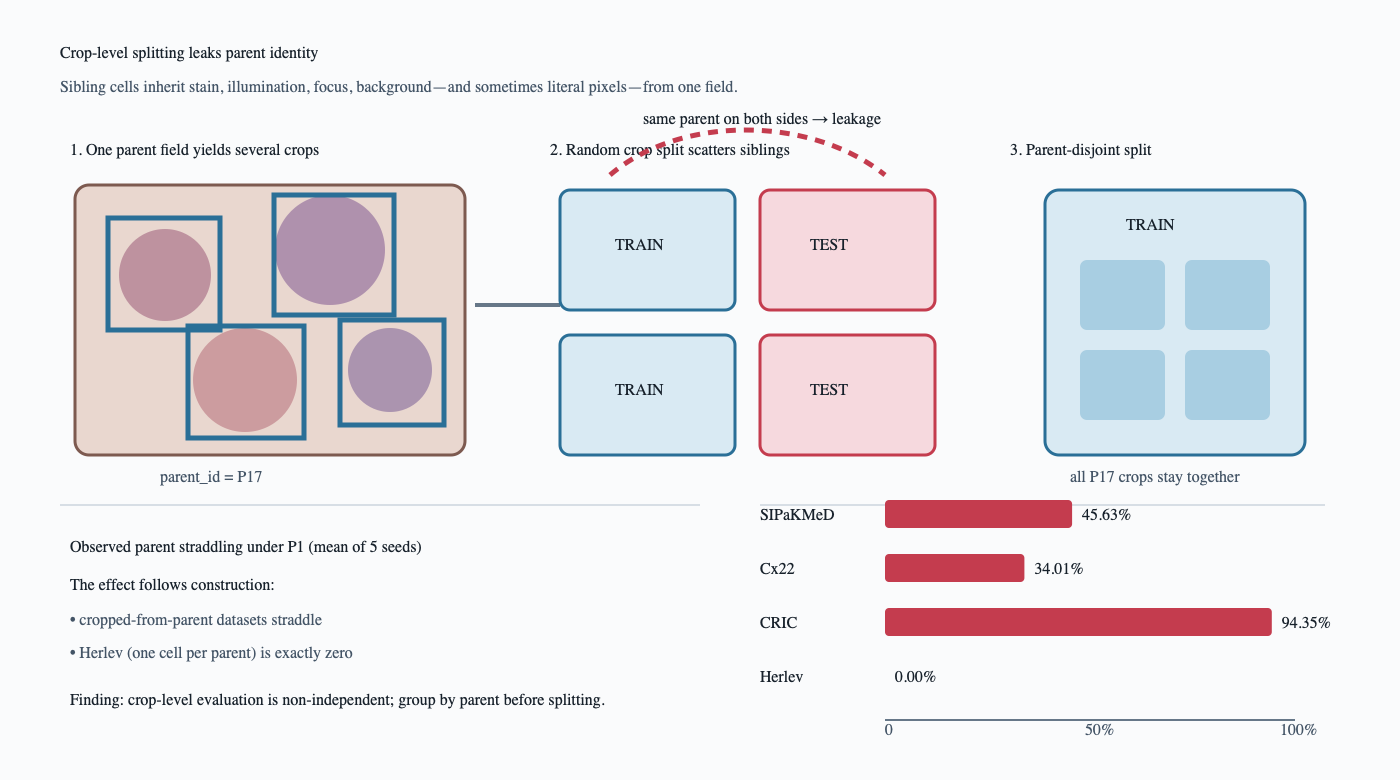
\includegraphics[width=0.96\textwidth]{figures/fig_leakage_schematic.png}
\caption{How crop-level splitting exposes parent identity. Sibling crops from one field inherit a common acquisition signature and, in 2,185 of 13,064 within-parent SIPaKMeD pairs, intersecting source coordinates; a random crop split scatters them across arms, whereas parent grouping keeps them together. Bars give observed \protocol{P1} straddle rates per dataset.}
\label{fig:schematic}
\end{figure*}

\subsection{Result 2: The Shortcut Is Learnable, and It Is Not the Cell}
Table~\ref{tab:probe} and Figure~\ref{fig:probe} report the probe.
On the balanced 424-way task, parent identity is recovered at \meanpm{25.73}{0.66}\%---109.1$\times$ the 0.2358\% chance baseline.
The shuffled-label control collapses to \meanpm{0.17}{0.24}\%, with a five-seed 95\% interval of $-0.14$\% to $0.47$\% that covers the exact chance value, confirming that the probe measures field identity rather than an artifact of the task construction.

Parent information survives every prespecified transformation: \meanpm{13.80}{1.12}\% under grayscale, \meanpm{17.31}{0.64}\% after stain normalization, \meanpm{16.27}{0.60}\% under high-pass filtering.
The decisive condition is background-only, which reaches \meanpm{18.68}{1.25}\%---79.2$\times$ chance from an image whose cell has been masked out and inpainted.
The fingerprint is therefore not cellular morphology but \emph{acquisition context}: slide preparation, illumination, focus, and debris field.

That is the generalizing observation of this paper.
Because the substrate is context rather than content, the exposure is a property of the \emph{construction}---any crop-level split of any cropped-from-field cytology release carries it, regardless of how carefully the class labels were assigned.
Persistence across all four transformations shows the signal is distributed rather than confined to one channel, and does not identify a single exclusive substrate.
Notably, stain normalization---the standard remedy for inter-slide appearance variation---leaves \meanpm{17.31}{0.64}\% recoverable, so it is not a sufficient defense against this exposure.

\begin{table}[t]
\caption{Parent-ID probe ablation on the balanced 424-way task. Chance is 0.2358\%.}
\label{tab:probe}
\centering
\scriptsize
\setlength{\tabcolsep}{4.2pt}
\begin{tabular}{lrr}
\toprule
Input condition & Accuracy & Multiple of chance \\
\midrule
RGB & \meanpm{25.73}{0.66}\% & 109.1$\times$ \\
Grayscale & \meanpm{13.80}{1.12}\% & 58.5$\times$ \\
Stain-normalized & \meanpm{17.31}{0.64}\% & 73.4$\times$ \\
Background only & \meanpm{18.68}{1.25}\% & 79.2$\times$ \\
High-pass & \meanpm{16.27}{0.60}\% & 69.0$\times$ \\
Shuffled labels & \meanpm{0.17}{0.24}\% & 0.7$\times$ \\
\bottomrule
\end{tabular}
\end{table}

\begin{figure}[t]
\centering
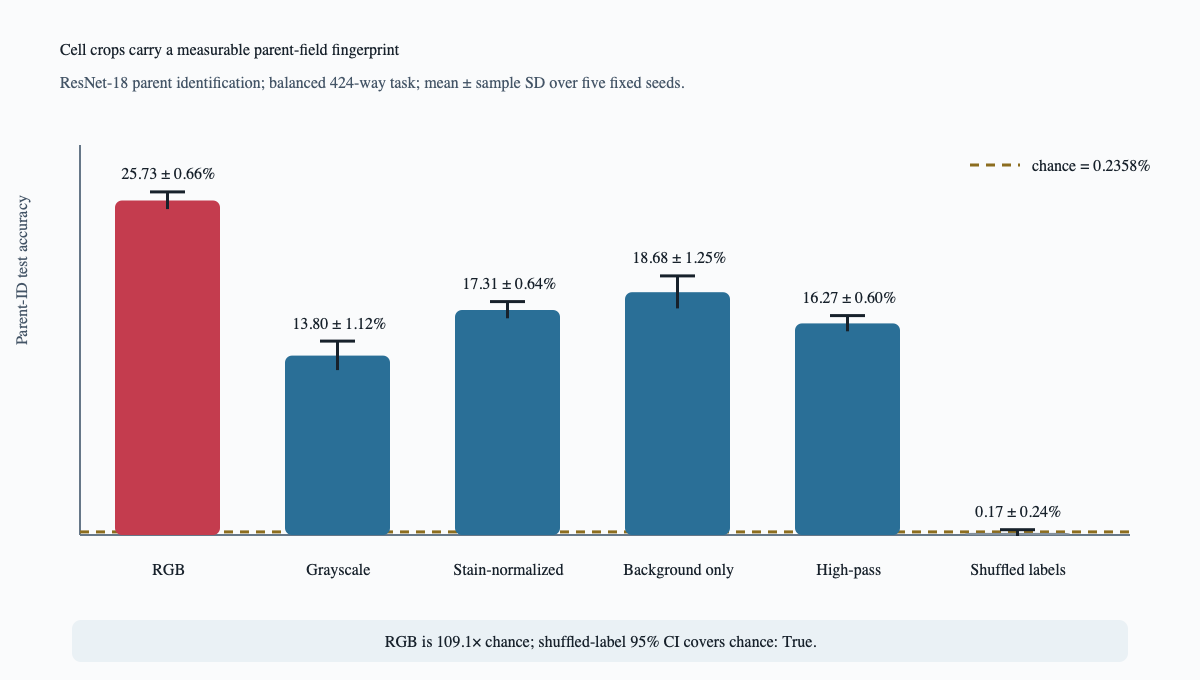
\includegraphics[width=\linewidth]{figures/fig_probe_ablation.png}
\caption{Parent-identity probe under four prespecified transformations and a shuffled-label control. Every transformed condition remains at least 58$\times$ chance; background-only inputs, from which the cell has been removed, still reach 79.2$\times$.}
\label{fig:probe}
\end{figure}

\subsection{Result 3: Bounded Accuracy Sensitivity}
Table~\ref{tab:classification} and Figure~\ref{fig:protocol} rescore six architectures on SIPaKMeD under identical training settings and identical 3,239/810 split sizes.
Correcting the evaluation unit lowers accuracy for \emph{every} architecture: \protocol{P1}$-$\protocol{P2} ranges from \meanpm{0.72}{0.83} points (ResNet-50) to \meanpm{2.25}{1.63} (MobileNet-V2), with a mean of 1.37 points across the six.
Because \protocol{P1$'$}=\protocol{P1} on SIPaKMeD, these differences cannot be attributed to a reduction in training-set size; the training and test counts are held exactly fixed across protocols.

Table~\ref{tab:inference} reports the preregistered paired inference.
Effect sizes are moderate to large ($d_z$ from 0.588 to 1.561), and five of six bootstrap intervals for $d_z$ exclude zero, but with five seeds and a declared 12-test Benjamini--Hochberg family no contrast survives adjustment; the smallest adjusted value is $q=0.1109$.
The design is therefore \emph{underpowered to certify individual architecture-wise contrasts}, which is a property of the sample size and correction breadth rather than evidence of absence.
We report the direction and scale of the protocol effect, and explicitly do not claim a confirmatory universal inflation effect.

\begin{table*}[t]
\caption{SIPaKMeD test accuracy. All models were rerun in this study under the same 3,239/810 train/test counts. Mean $\pm$ sample SD over five seeds.}
\label{tab:classification}
\centering
\scriptsize
\setlength{\tabcolsep}{7pt}
\begin{tabular}{lrrrr}
\toprule
Architecture & \protocol{P1} crop & \protocol{P1$'$} size-matched & \textbf{\cytofair{} \protocol{P2} parent-disjoint} & \protocol{P3} component-disjoint \\
\midrule
DenseNet-121 & \meanpm{98.12}{0.28}\% & \meanpm{98.12}{0.28}\% & \textbf{\meanpm{96.72}{0.69}\%} & \meanpm{97.38}{0.50}\% \\
EfficientNet-B0 & \meanpm{97.78}{0.49}\% & \meanpm{97.78}{0.49}\% & \textbf{\meanpm{96.69}{1.49}\%} & \meanpm{97.41}{0.71}\% \\
MobileNet-V2 & \meanpm{97.41}{0.45}\% & \meanpm{97.41}{0.45}\% & \textbf{\meanpm{95.16}{1.50}\%} & \meanpm{96.20}{0.93}\% \\
ResNet-18 & \meanpm{97.19}{0.59}\% & \meanpm{97.19}{0.59}\% & \textbf{\meanpm{96.00}{0.89}\%} & \meanpm{96.35}{1.28}\% \\
ResNet-50 & \meanpm{97.51}{0.47}\% & \meanpm{97.51}{0.47}\% & \textbf{\meanpm{96.79}{0.42}\%} & \meanpm{96.27}{0.53}\% \\
ViT-B/16 & \meanpm{97.14}{0.95}\% & \meanpm{97.14}{0.95}\% & \textbf{\meanpm{95.56}{0.84}\%} & \meanpm{95.53}{1.68}\% \\
\bottomrule
\end{tabular}
\end{table*}

\begin{table*}[t]
\caption{Preregistered paired \protocol{P1}$-$\protocol{P2} inference. $\Delta$ is percentage points, $d_z$ is paired Cohen's effect, and $q$ is BH-adjusted over the declared 12-test family.}
\label{tab:inference}
\centering
\scriptsize
\setlength{\tabcolsep}{7.0pt}
\begin{tabular}{lrrrrr}
\toprule
Architecture & $\Delta$, mean $\pm$ SD & Raw $p$ & BH $q$ & Cohen's $d_z$ & Bootstrap 95\% CI for $d_z$ \\
\midrule
DenseNet-121 & \meanpm{1.41}{0.90} & 0.0251 & 0.1109 & 1.561 & [0.985, 4.747] \\
EfficientNet-B0 & \meanpm{1.09}{1.85} & 0.2591 & 0.2591 & 0.588 & [$-0.316$, 4.668] \\
MobileNet-V2 & \meanpm{2.25}{1.63} & 0.0370 & 0.1109 & 1.377 & [0.809, 6.686] \\
ResNet-18 & \meanpm{1.19}{1.28} & 0.1081 & 0.1511 & 0.922 & [0.442, 2.365] \\
ResNet-50 & \meanpm{0.72}{0.83} & 0.1260 & 0.1511 & 0.863 & [0.085, 4.025] \\
ViT-B/16 & \meanpm{1.58}{1.70} & 0.1059 & 0.1511 & 0.931 & [0.057, 4.950] \\
\bottomrule
\end{tabular}
\end{table*}

\begin{figure}[t]
\centering
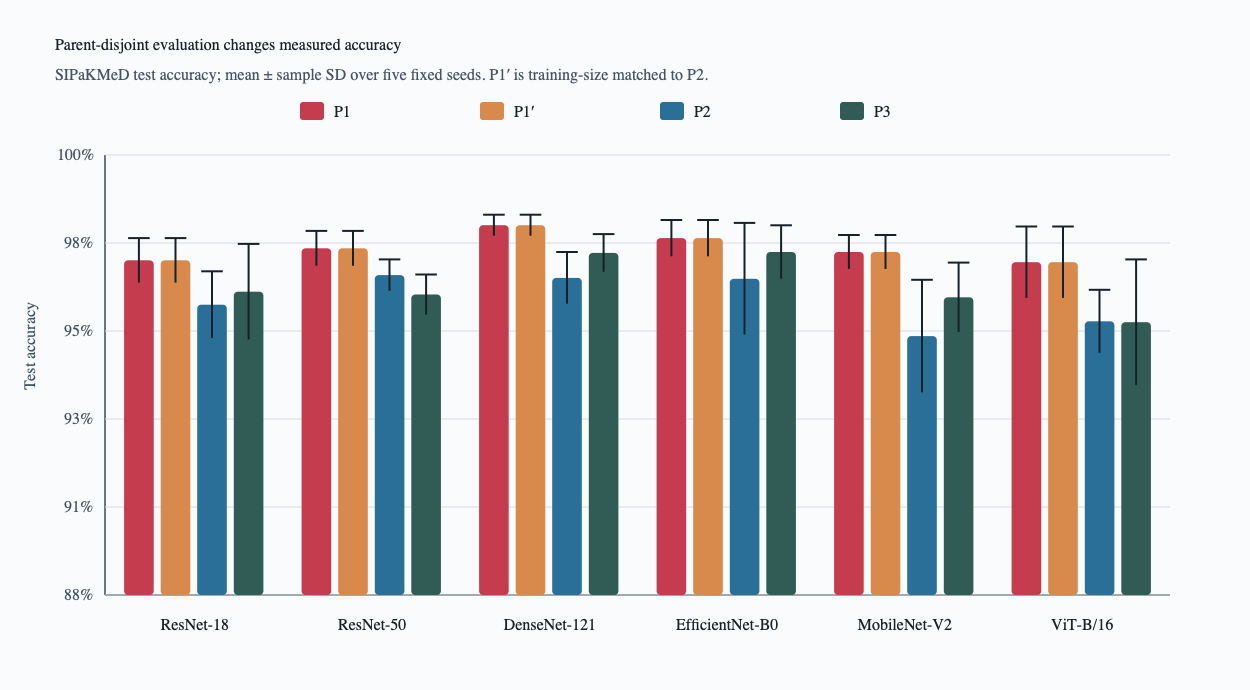
\includegraphics[width=\linewidth]{figures/fig_protocol_accuracy.png}
\caption{SIPaKMeD accuracy across all four protocols. \protocol{P1$'$} is exactly \protocol{P1} because the random split already carries the \protocol{P2} training volume, so the \protocol{P1}$\rightarrow$\protocol{P2} drop cannot be attributed to training-set size.}
\label{fig:protocol}
\end{figure}

\subsection{Result 4: Parent Grouping Is Sufficient}
\label{sec:p2p3}
Table~\ref{tab:p2p3} reports the secondary \protocol{P2}$-$\protocol{P3} contrast, which is outside the confirmatory family and reported unadjusted.
No architecture shows a detectable difference: the smallest unadjusted $p$ is 0.0971, four of six point estimates favor \protocol{P3} and two favor \protocol{P2}, and five of six bootstrap intervals for $d_z$ span zero.

The interpretation is practical.
\protocol{P3} adds perceptual-hash near-duplicate merging on top of exact parent grouping, at meaningful implementation and computational cost.
That extra conservatism buys no measurable change, which indicates the hash-connected components largely capture within-parent structure that \protocol{P2} has already absorbed.
For practitioners constructing corrected splits on releases of this kind, grouping by recovered parent appears sufficient, and the similarity-purging stage can be treated as optional.

\begin{table}[t]
\caption{Secondary \protocol{P2}$-$\protocol{P3} contrast, unadjusted. No architecture shows a detectable difference.}
\label{tab:p2p3}
\centering
\scriptsize
\setlength{\tabcolsep}{3.6pt}
\begin{tabular}{lrrrr}
\toprule
Architecture & $\Delta$, mean $\pm$ SD & Unadj. $p$ & $d_z$ & 95\% CI for $d_z$ \\
\midrule
DenseNet-121 & \meanpm{$-0.67$}{0.69} & 0.0971 & $-0.965$ & [$-3.266$, $-0.725$] \\
EfficientNet-B0 & \meanpm{$-0.72$}{1.94} & 0.4562 & $-0.369$ & [$-2.708$, 0.467] \\
MobileNet-V2 & \meanpm{$-1.04$}{1.38} & 0.1673 & $-0.753$ & [$-3.329$, 0.075] \\
ResNet-18 & \meanpm{$-0.35$}{1.19} & 0.5510 & $-0.291$ & [$-1.516$, 1.255] \\
ResNet-50 & \meanpm{0.52}{0.66} & 0.1545 & 0.784 & [0.361, 2.534] \\
ViT-B/16 & \meanpm{0.02}{2.34} & 0.9823 & 0.011 & [$-3.338$, 0.817] \\
\bottomrule
\end{tabular}
\end{table}

\subsection{Registered Predictions and What They Rule Out}
Two preregistered predictions were not supported, and both are retained.

First, the monotonic ordering \protocol{P3}$\leq$\protocol{P2}$\leq$\protocol{P1} fails for four of six architectures (Table~\ref{tab:ordering}).
On inspection the prediction was mis-specified rather than falsified: \protocol{P3} merges parents into similarity-connected components and therefore changes grouped \emph{test composition}, so it is not nested within \protocol{P2} and no monotone finite-sample ordering should have been expected.
Section~\ref{sec:p2p3} shows the difference is undetectable in either direction, which is the substantive reading.

Second, ranking stability cannot be resolved at this sample size.
Kendall's $\tau$ between \protocol{P1} and \protocol{P2} architecture orderings is 0.467 with 4/15 pairwise reversals and no tie changes, but the seed-bootstrap 95\% CI spans 0.071--0.733 and the unadjusted $p=0.2722$; with six architectures this is indistinguishable from chance and we draw no conclusion from it.

Finally, a scope note on the frozen evidence.
The run schema retained aggregate accuracy, macro-F1, balanced accuracy, and epoch histories, but not final per-sample predictions or checkpoints.
A post-hoc class confusion matrix would require new inference after the declared hard stop; we neither fabricate one nor infer class-pair errors from aggregate metrics.
Figure~\ref{fig:loss} shows the retained optimization diagnostic: training loss converges under both protocols, so the accuracy gap in Table~\ref{tab:classification} is not an optimization failure under \protocol{P2}.

\begin{table}[t]
\caption{Registered protocol-ordering diagnostic. \protocol{P3} is not nested within \protocol{P2}; see Section~\ref{sec:p2p3}.}
\label{tab:ordering}
\centering
\scriptsize
\begin{tabular}{lc}
\toprule
Architecture & \protocol{P3}$\leq$\protocol{P2}$\leq$\protocol{P1} \\
\midrule
DenseNet-121 & Not supported \\
EfficientNet-B0 & Not supported \\
MobileNet-V2 & Not supported \\
ResNet-18 & Not supported \\
ResNet-50 & Supported \\
ViT-B/16 & Supported \\
\bottomrule
\end{tabular}
\end{table}

\begin{figure}[t]
\centering
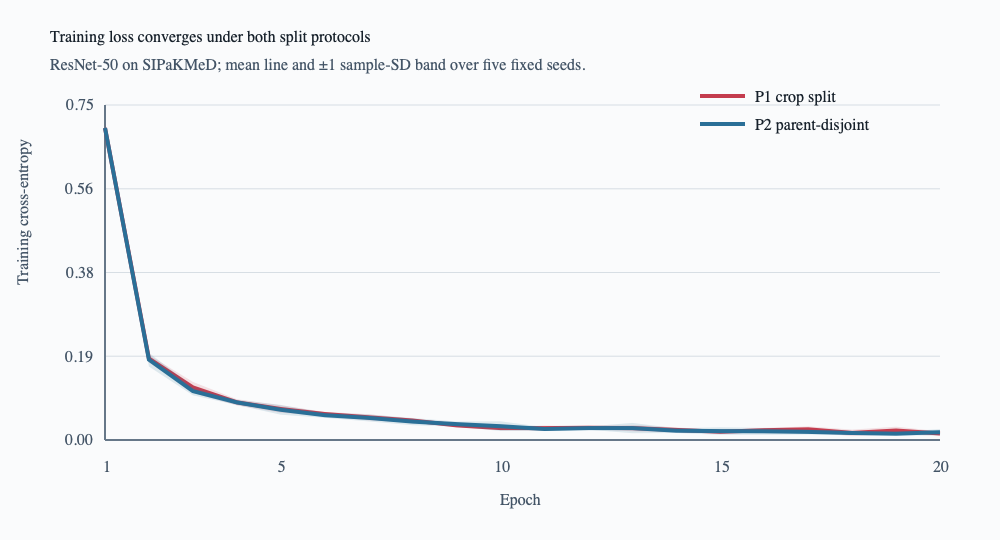
\includegraphics[width=0.82\linewidth]{figures/fig_loss_curves.png}
\caption{Frozen ResNet-50 training-loss histories under \protocol{P1} and \protocol{P2}. Both converge, so the protocol accuracy difference is not an optimization artifact.}
\label{fig:loss}
\end{figure}

\section{Discussion}
\subsection{What Is Established}
The finding is structural rather than architectural.
For three of four audited benchmarks the released image is not the independent sampling unit, and this is now a recovered and doubly validated fact rather than a conjecture: two independent recoveries agree on 4,049/4,049 SIPaKMeD crops, the observed straddle rates reproduce an analytic prediction, and a single-cell control returns exactly zero.
Under the protocol the literature uses, most SIPaKMeD test crops have a training parent and more than half share literal source pixels with a training crop.
The signal that links them is learnable at 109$\times$ chance, and at 79$\times$ chance after the cell itself is removed.

\subsection{Does It Matter? A Calibration}
The natural objection is that a 1.37-point mean accuracy change is small.
It is small in absolute terms and large relative to the quantity the field is contesting.
The two strongest published five-class SIPaKMeD results we cite differ by 0.62 points~\cite{rahaman2021deepcervix,gao2022knowledge}.
Our measured protocol effect exceeds that spread for \emph{every} architecture tested---the smallest, ResNet-50 at \meanpm{0.72}{0.83} points, still exceeds it---and reaches 2.25 points, roughly 3.6$\times$ the published spread, for MobileNet-V2.

This is a comparison of \emph{magnitudes}, not of accuracies.
We deliberately do not place our numbers alongside published numbers, because different splits do not define comparable tests.
What is comparable is the sensitivity of a fixed pipeline to the split protocol, set against the size of the differences the literature reports.
On that comparison, protocol choice is not a second-order detail on these benchmarks: it is of the same order as, or larger than, the methodological progress being claimed.

\subsection{What Is Not Established}
We show that a shortcut is available, not that classifiers use it.
The probe demonstrates that field identity is recoverable from a crop; it does not demonstrate that a class model routes its prediction through that identity, and our frozen evidence cannot settle the question.
Establishing consequence---as distinct from availability---requires a causal design such as intervention on the fingerprint substrate, and remains open.

Interpretation of the weakest architecture--protocol cells, MobileNet-V2 under \protocol{P2} (\meanpm{95.16}{1.50}\%) and ViT-B/16 under \protocol{P3} (\meanpm{95.53}{1.68}\%), must remain aggregate, since no class confusion matrix exists in the frozen artifacts.
Two dataset properties nevertheless make composition sensitivity expected without invoking a specific error pair: crop counts are nearly balanced (787--831 per class) while parent counts range from 108 to 271, and cervical categories are defined by related morphological criteria rather than separated acquisition domains.
A parent-disjoint fold can therefore preserve crop totals while altering the diversity of independently sourced appearances.

\subsection{Threats to Validity}
Three alternative explanations deserve explicit treatment.

\emph{A split-implementation bug.}
This would have to reproduce an analytic prediction it was never given, return exactly zero on the one dataset whose construction forbids leakage, and scale monotonically with crop-per-parent ratio across three others.
Dual-branch recovery, the Monte Carlo interval check, and the Herlev control are mutually independent, and a single bug is unlikely to satisfy all three.

\emph{A degenerate probe task.}
If the probe were exploiting task construction rather than image content, the shuffled-label control would not collapse to a five-seed interval covering exact chance.
It does.

\emph{Reduced effective training diversity rather than removed leakage.}
\protocol{P2} preserves crop counts exactly but necessarily changes which parents appear in training, so part of the accuracy change may reflect appearance diversity rather than removed shortcut access.
We cannot separate these components with the present design, and we do not claim to; \protocol{P1$'$} rules out the training-\emph{volume} explanation only.

\subsection{A Design Lesson We Record Rather Than Repair}
The scientific question here was singular---does crop-level splitting inflate reported accuracy---but the preregistered analysis tested it six times, once per architecture, and then paid a six-way multiplicity penalty for asking once per backbone.
A pooled omnibus endpoint treating architecture as a nuisance factor would have addressed the same question at materially higher power.
We did not preregister one, and we therefore do not substitute one after seeing the results; we record the mis-specification so that the replication described in Section~\ref{sec:conclusion} can be designed correctly.

\section{Recommendations}
The measurements support four concrete recommendations for anyone building or consuming cropped-from-field cytology benchmarks.

\emph{Release the parent identifier.}
Most of the exposure documented here exists because the crop-to-field mapping was not carried into the released folder structure. Publishing a single provenance column costs nothing and makes correct grouping the default rather than a research project.

\emph{Group by parent, and stop there.}
Section~\ref{sec:p2p3} finds no detectable benefit from adding perceptual-hash component merging on top of exact parent grouping. Exact provenance is both cheaper and sufficient.

\emph{Do not rely on stain normalization as a defense.}
Parent identity remains recoverable at \meanpm{17.31}{0.64}\% after channel-statistics matching, so appearance normalization does not remove the acquisition fingerprint.

\emph{State the split unit, and report seed variance.}
Reported differences on these benchmarks are of the same order as the protocol effect and as seed-to-seed variation. A single accuracy figure without a stated grouping unit and a dispersion estimate is not interpretable.

\subsection{Self-Audit and Scope}
This is a resource and measurement study.
Affected prior results are discussed in aggregate, and no individual publication is labeled deficient; the protocols in question were standard practice, and the released datasets did not make the alternative convenient.
The audit scope includes the present authors' own prior work on these benchmarks, which is subject to the same correction as any other.
Grouped scores are estimates at a more defensible deployment unit, and a lower apparent score does not imply lower clinical utility.

\section{Limitations}
The audited public datasets are modest in independent-parent count, and only SIPaKMeD received the complete six-architecture rescore; Cx22, CRIC, and Herlev receive structural audits alone.
Claims about the magnitude of downstream performance change are therefore restricted to one benchmark.
The per-architecture inference is underpowered at five seeds under a 12-test family, so the accuracy arm estimates rather than certifies.
The \protocol{P2}$-$\protocol{P3} null is likewise a failure to detect a difference at this sample size, not a demonstration of equivalence; a formal equivalence test was not preregistered.
No prospective clinical validation, patient-level outcome study, or deployment analysis was performed, and the corrected benchmark scores must not be read as estimates of clinical utility.
Training was constrained to at most three RTX A6000 GPUs, which limited broader full-matrix reruns, and the frozen aggregate artifacts cannot support a post-hoc class confusion matrix without violating the declared hard stop.

\section{Conclusion}
\label{sec:conclusion}
We asked whether public cervical-cytology classifiers are evaluated on genuinely independent cells, and found that released crop filenames conceal a consequential source-field hierarchy.
\cytofair{} recovers that hierarchy exactly, validates it by two independent routes, and measures what crop-level splitting shares.
On SIPaKMeD, \meanpm{92.62}{0.40}\% of test crops have a training parent and \meanpm{52.62}{1.97}\% share literal source pixels with a training crop; CRIC reaches \meanpm{99.97}{0.08}\%; single-cell Herlev returns exactly zero and validates the instrument.
Cx22 is the instructive intermediate case: its official Multi split is already parent-disjoint, and the exposure appears only when the Pair subset is pooled with it.

The shared signal is learnable at 109$\times$ chance and at 79$\times$ chance from inpainted background alone, locating it in acquisition context rather than cell morphology---which makes the exposure a property of the cropped-from-field construction itself rather than of any labeling decision.
Correcting the evaluation unit reduces accuracy for all six architectures tested, by a mean of 1.37 points, exceeding the 0.62-point spread between the two strongest published results, although our five-seed per-architecture design cannot certify individual contrasts after multiplicity correction.
Adding near-duplicate purging on top of parent grouping changes nothing detectable, so the cheaper correction suffices.
The contribution is accordingly a benchmark correction and a reusable measurement resource---exact provenance maps, fixed parent-disjoint splits, and the audit toolkit---rather than another incremental classifier.

Two extensions follow directly and are already specified.
A preregistered, adequately powered replication with a single pooled endpoint, replacing the per-architecture family that this study recorded as mis-specified, and a causal decomposition of the effect are in progress (registered as \texttt{PREREGISTRATION\_STUDY2.md} in the repository).
We will then extend the same grouping apparatus to provenance-aware instance segmentation on Cx22, and to two constructions whose grouping units are known in advance but never enforced: specimen-disjoint multi-view Fish-Pak and temporally grouped Croatian Fish video, with deterministic manifests fixed before any model is trained.

\bibliographystyle{IEEEtran}
{\scriptsize\bibliography{references}}

\end{document}
